\chapter{Lec 12 - Reduction}

\section{NP-Hardness (formal definition)}
\textbf{Definition:}\newline
A problem $A$ \textbf{reduces} in polynomial time to problem $B$ ($A <_p B$) if exists a polynomial time algorithm that transforms an arbitrary input instance $a$ of $A$ into an input instance $b$ of $B$ such that:
\begin{enumerate}
    \item if $a$ is a YES instance of $A$, then $b$ is a YES instance of $B$
    
    \item if $b$ is a YES instance of $B$, then $a$ is a YES instance of $A$ 
\end{enumerate}
\textbf{Property:}\newline
$A <_p B$ and $B <_p C \rightarrow A <_p C$\newline\newline
Now we can give a more formal definition of \textbf{NP-Hardness}:\newline
A problem is \textbf{NP-Hard} if every problem in \textbf{NP} reduces in polynomial time to it.\newline\newline
Then, to prove that a problem $X$ is \textbf{NP-Hard}, we can reduce a known \textbf{NP-Hard} problem $Y$ (e.g. 3SAT) to $X$. Note that NP-Hardness \textbf{does not} mean that the problem is not in $P$, it provides a strong evidence for that.

\section{NP-Hardness proof}
\textbf{Theorem:} TSP is \textbf{NP-Hard}\newline\newline
\textbf{Proof:}\newline
Reduction from Hamiltonian circuit to TSP ($Ham. <_p TSP$). Since TSP is not a decision problem, we have to redefine it.\newline\newline
\textbf{TSP:}
\begin{itemize}
    \item \textbf{input:} $G=(V, E)$ complete, undirected, weighted graph, $k \in \mathbb{R}$

    \item \textbf{output:} $\exists$ in $G$ a Hamiltonian circuit of cost at most $k$ ($\leq k$).
\end{itemize}
Pick an arbitrary input instance for Ham. and create the following input for TSP: $G'(V, E')$ complete, undirected, weighted graph with:
\[w(e \in E') = \left\{\begin{array}{lr}
                    1 & \text{if } e \in E \\
                    \infty & \text{otherwise}
                \end{array}\right\}\]

If we set $k=n$ the following holds:
\begin{enumerate}
    \item if $G$ has an Hamiltonian circuit, then the TSP algorithm run on $G'$ returns an Hamiltonian circuit of cost $n$

    \item if $G$ doesn't have an Hamiltonian circuit, then any Hamiltonian circuit in $G'$ must have at least one edge not in $G$, hence of weight $\infty$. In this case a TSP algorithm run on $G'$ returns an Hamiltonian circuit of cost $> n$.
\end{enumerate}
If we had a fast algorithm for TSP we would solve also the Hamiltonian circuit problem.

\section{Maximum Independent Set}
\textbf{Independent set:}
 Given a graph $G=(V,E)$, an independent set in $G$ is a set $I \subseteq V$ with no edges between them.\newline\newline
\textbf{Maximum independent set problem:} compute an independent set of maximum size.\newline\newline
\textbf{Theorem:} Maximum Independent set is \textbf{NP-hard}\newline\newline
\textbf{Proof:}\newline
Reduction from 3SAT to maximum independent set. 
\begin{center}
    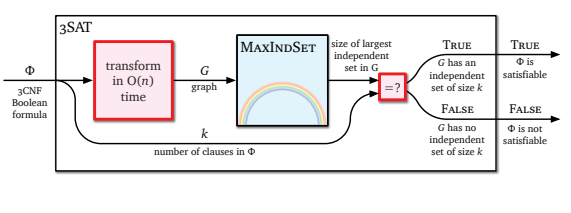
\includegraphics[]{images/Reduction max ind set.png}
\end{center}
Pick an arbitrary 3CNF boolean formula $f$ with $k$ clauses:
\[(a \lor b \lor c) \land (b \lor \neg{c} \lor \neg{d}) \land (\neg{a} \lor c \lor d) \land (a \lor \neg{b} \lor \neg{d})\]
We define a graph starting from $f$:
\begin{itemize}
    \item Vertices: Each vertex represents one literal in $f$. A \textit{group} of 3 vertices represents a clause.
    \item Edges: Edges is $E$ are of two types:
    \begin{enumerate}
        \item We add an edge between a literal and its inverse, for all the literals.

        \item We add an edge between every pair of vertices that are in the same group.
    \end{enumerate}
    \begin{center}
        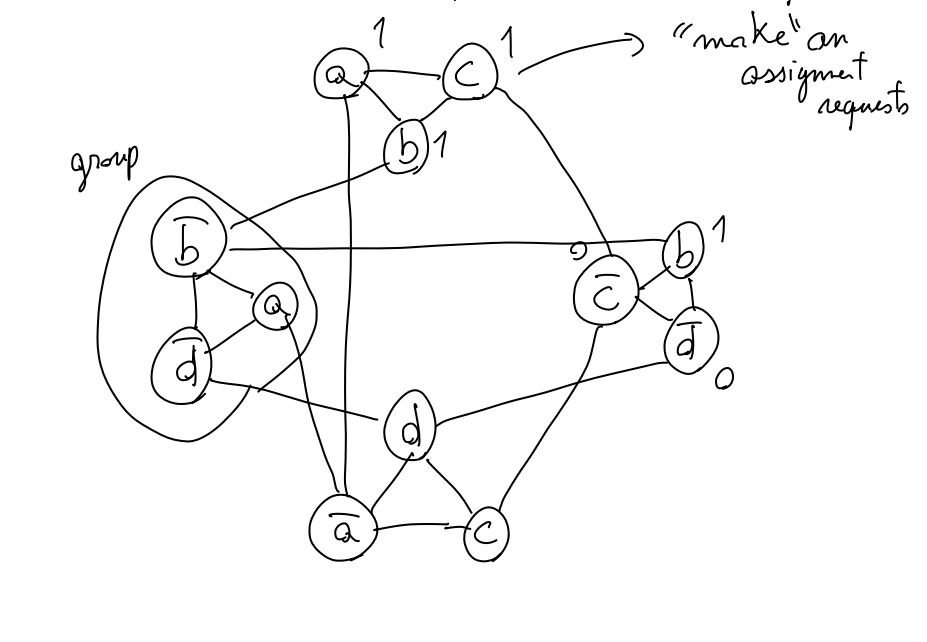
\includegraphics[scale=0.7]{images/Max Ind Set.png}
    \end{center}
\end{itemize}
Suppose we assign the value true to each literal, then, an edge connects two vertices that are either in the same group or that are \textit{asking} for inconsistent assignment for the same variable. Therefore, an independent set is forced to select at most one vertex per group (the largest independent set in G has size at most $k$). If $G$ contains an independent set of size exactly $k$ (number of clauses), the formula $f$ is satisfiable.\newline\newline
\textbf{Formal proof:}\newline
\textbf{Claim} : $G$ contains an independent set of size exactly $k$ $\iff$ the formula $f$ is satisfiable. \newline\newline
\textbf{Proof:}
\begin{itemize}
    \item $\Rightarrow$: Suppose $f$ is satisfiable.  Fix an arbitrary satisfying assignment. By definition, each clause contains at least one true literal.Choose a subset $S$ of $k$ vertices in $G$ that contains exactly one vertex per group, such that the corresponding $k$ literals are all true. Then, $S$ is an independent set of size $k$ because it does not contain both endpoints of any edge of a group, nor of any edge that connects inconsistent literals.

    \item $\Leftarrow$: Suppose $G$ contains an independent set $S$ of size $k$. Each vertex in $S$ must lie in a different group. Suppose we assign the value true to each literal in $S$. Since inconsistent literals are connected by an edge , this assignment is consistent. Since $S$ contains one vertex per group, each clause in $f$ contains (at least) one true literal. This implies that $f$ is satisfiable.
\end{itemize}

